\centering
\begin{table}
	\begin{tabular}{cc>{\raggedright\arraybackslash}p{5.5cm}}
		\toprule \multicolumn{1}{c}{\textbf{}}                                           & \multicolumn{1}{c}{\textbf{Turn}} & \multicolumn{1}{c}{\textbf{Description}}         \\
		\midrule \rowcolor{gray!10} 
\includegraphics[scale=0.07]{figs/emojis/mini_1.png} & 0                                 & Target Navigation Effectiveness                  \\
		\midrule \rowcolor{gray!10} 
\includegraphics[scale=0.07]{figs/emojis/mini_2.png} & 0                                 & Efficient Exploration and Map Memory Utilization \\
		\midrule \rowcolor{gray!10} 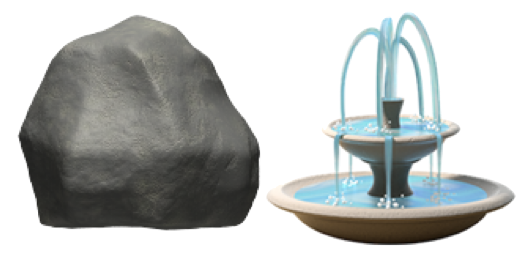
\includegraphics[scale=0.07]{figs/emojis/mini_3.png} & 0                                 & Hazard Awareness and Equipment Utilization       \\
		\midrule \rowcolor{gray!10} 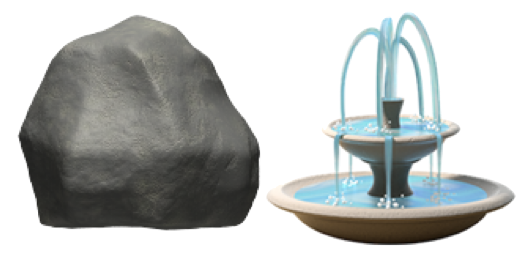
\includegraphics[scale=0.07]{figs/emojis/mini_4.png} & 0                                 & Boulder Manipulation Strategy                    \\
		\midrule \rowcolor{gray!10} 
\includegraphics[scale=0.07]{figs/emojis/mini_5.png} & 0                                 & Combat Engagement and Survival                   \\
		\midrule \rowcolor{gray!10} 
\includegraphics[scale=0.07]{figs/emojis/mini_6.png} & 0                                 & Role-Specific Ability Utilization                \\
		\midrule \rowcolor{gray!30} 
\includegraphics[scale=0.07]{figs/emojis/mini_7.png} & 1                                 & Spatial Awareness and Interpretation             \\
		\midrule \rowcolor{gray!30} 
\includegraphics[scale=0.07]{figs/emojis/mini_8.png} & 1                                 & Object Pickup Efficiency                         \\
		\midrule \rowcolor{gray!60} 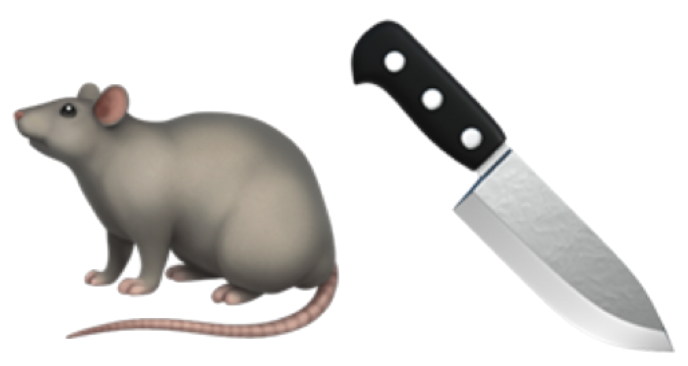
\includegraphics[scale=0.07]{figs/emojis/mini_9.png} & 2                                 & Giant Rats Encounter Handling                    \\
		\bottomrule
	\end{tabular}
	\caption{\raggedright Metrics and Turn of Induction for MiniHack}
	\label{tab:metrics_mini}
\end{table}